\documentclass[11pt,a4paper]{article}

\usepackage[margin=2.4cm]{geometry}
\usepackage{amsmath,amssymb,amsthm}
\usepackage{booktabs}
\usepackage{graphicx}
\usepackage{hyperref}

\newtheorem{theorem}{Theorem}
\newtheorem{corollary}{Corollary}
\newtheorem{proposition}{Proposition}
\newtheorem{definition}{Definition}
\newtheorem{remark}{Remark}

\newcommand{\F}{\mathbb{F}}
\newcommand{\Z}{\mathbb{Z}}
\newcommand{\ket}[1]{|#1\rangle}
\newcommand{\bra}[1]{\langle#1|}

\title{\textbf{Modular Walsh Rigidity and Antipodal Obstructions for Flat Non-Clifford Hypergraph States}}

\author{
  Filipe Martins Vono \and
  Andr\'e Oliveira Naufel de Toledo \and
  Val\'eria Gonzaga Santos
}

\date{November 19, 2026}

\begin{document}
\maketitle

\begin{abstract}
Hypergraph states prepared by diagonal non-Clifford phase circuits $\{Z, CZ, CCZ, CCCZ\}$ correspond directly to Boolean functions $f:\F_2^n\to\F_2$ of algebraic degree at most four, and the native $n$-qubit Hadamard layer $H^{\otimes n}$ maps their computational-basis phases to the Walsh--Hadamard spectrum $W_f(b)$. We translate two recent structural theorems on Boolean bent functions into practical certification and synthesis results for flat (bent) hypergraph states. First, from the Lean-certified universal antipodal necessity theorem for rotation-symmetric Boolean functions of degree at most three, we obtain an exact topological obstruction for ring architectures: no rotation-symmetric $\{Z, CZ, CCZ\}$ circuit on $n=2H$ qubits can prepare a flat hypergraph state without the full antipodal $CZ$ orbit $\{(i, i+H)\}$, ruling out local-range ring ans\"atze and pure-$CCZ$ symmetric circuits and imposing a lower bound of $\lceil H(H-1)/2 \rceil$ SWAPs ($3\lceil H(H-1)/2 \rceil$ CNOTs) on nearest-neighbor 1D rings. Second, from uniform ($8/15$ for all $m\ge 4$) and asymptotic ($1/2$ for sufficiently large $m$) modular Walsh rigidity for degree-four Boolean functions on $n=4m$ qubits, we derive an overflow-free \texttt{uint8} modular certification algorithm that verifies exact $X$-basis flatness using arithmetic modulo a single odd integer $p \approx 2^{n/4}$ rather than full $O(n/2)$-bit precision. We prove an explicit universal degree-four counterexample family that passes modulo $p=3$ with zero violations across all $2^n$ frequencies despite being $100\%$ non-flat, showing why a rigidity threshold is essential. Numerical benchmarks in Python/NumPy up to $n=28$ qubits ($268{,}435{,}456$ amplitudes, $p=69$) confirm $4\times$ memory reduction ($256\,\text{MB}$ vs.\ $1024\,\text{MB}$) and $1.35\times$ speedup. Scaling with a multi-threaded C/OpenMP engine on cloud nodes reaches $n=32$ qubits ($4.29 \times 10^9$ amplitudes, $p=137$) in $13.67\,\text{s}$ vs.\ $19.74\,\text{s}$ ($1.44\times$ faster, $8\,\text{GB}$ vs.\ $16\,\text{GB}$ \texttt{int32} / $64\,\text{GB}$ \texttt{complex128}), and certifies \textbf{$n=36$ qubits ($6.87 \times 10^{10}$ amplitudes, $p=275$) in $141.57\,\text{s}$ ($128\,\text{GB}$ \texttt{uint16}) on a single $12$-vCPU, $160\,\text{GB}$ VM where exact \texttt{int32} ($256\,\text{GB}$) runs out of memory and \texttt{complex128} requires $1\,\text{TB}$}, alongside $100\%$ compilation-fault detection and non-Clifford magic up to $0.638\,n$ bits.
\end{abstract}

\section{Introduction}
Diagonal quantum phase circuits generated by multi-controlled-$Z$ gates $\{Z, CZ, CCZ, CCCZ\}$ sit at levels $\mathcal{C}_1$ through $\mathcal{C}_4$ of the Clifford hierarchy~\cite{Gottesman1999,Cui2017} and prepare the family of \emph{quantum hypergraph states}~\cite{Rossi2013,Qu2013,Gachechiladze2019}. Unlike stabilizer (graph) states prepared by $\{Z, CZ\}$ alone, hypergraph states of degree three and four possess genuine non-stabilizerness (\emph{magic})~\cite{Leone2022}, making them key resources for measurement-based quantum computation, quantum advantage protocols, and magic-state distillation.

A distinguished subclass consists of \emph{flat} (or \emph{bent}) hypergraph states: states $\ket{\psi_f}$ whose $X$-basis measurement distribution $|\bra{b}H^{\otimes n}\ket{\psi_f}|^2 = 2^{-n}$ is exactly uniform. Because $H^{\otimes n}$ implements the normalized Walsh--Hadamard transform natively on $n$ qubits, flatness of $\ket{\psi_f}$ is equivalent to the phase polynomial $f:\F_2^n\to\F_2$ being a \emph{bent function}~\cite{Carlet2021}, a connection also exploited in quantum algorithms for hidden bent functions~\cite{Rotteler2010}.

In this paper we bridge two recent mathematical results on bent functions---universal antipodal necessity~\cite{Vono2026Antipodal} and modular Walsh rigidity at thresholds $8/15$ and $1/2$~\cite{Vono2026Rigidity}---into two immediately applicable tools for quantum circuit synthesis and verification:
\begin{enumerate}
  \item \textbf{Topological synthesis obstruction in ring architectures (Section~\ref{sec:antipodal}):} an exact no-go theorem forbidding local-range or pure-$CCZ$ rotation-symmetric circuits of degree $\le 3$ from preparing flat hypergraph states on $n=2H$ qubits, together with explicit 1D-ring SWAP and CNOT routing lower bounds.
  \item \textbf{Compact modular flatness certification (Section~\ref{sec:modular}):} an overflow-free \texttt{uint8} arithmetic verification protocol for $\{Z, CZ, CCZ, CCCZ\}$ circuits on $n=4m$ qubits that halves the required bit-width ($\approx n/4$ bits instead of $n/2$ bits), cuts working memory by $4\times$ up to $n=28$ qubits, and mathematically guarantees zero false positives.
\end{enumerate}

\section{Preliminaries}
Let $f:\F_2^n\to\F_2$ be a Boolean function written in algebraic normal form (ANF) as
\[
  f(x) = \bigoplus_{S \in \mathcal{E}} \prod_{i \in S} x_i,
\]
where $\mathcal{E}$ is a collection of subsets of $\{0, \dots, n-1\}$ (a hypergraph) with $\max_{S \in \mathcal{E}} |S| = \deg(f)$. The associated diagonal phase unitary is
\[
  U_f = \prod_{S \in \mathcal{E}} C^{|S|-1}Z_S,
\]
and the corresponding \emph{hypergraph state} is
\[
  \ket{\psi_f} = U_f H^{\otimes n}\ket{0^n} = \frac{1}{\sqrt{2^n}} \sum_{x \in \F_2^n} (-1)^{f(x)}\ket{x}.
\]
Applying a final Hadamard layer $H^{\otimes n}$ yields
\[
  H^{\otimes n}\ket{\psi_f} = \frac{1}{2^n}\sum_{b \in \F_2^n} W_f(b)\ket{b},
  \qquad
  W_f(b) = \sum_{x \in \F_2^n} (-1)^{f(x) \oplus b\cdot x}.
\]

\begin{definition}[Flat Hypergraph State]
For even $n$, $\ket{\psi_f}$ is \emph{flat} (or \emph{bent}) if $|\bra{b}H^{\otimes n}\ket{\psi_f}|^2 = 2^{-n}$ for every $b \in \F_2^n$, equivalently $|W_f(b)| = 2^{n/2}$ for all $b \in \F_2^n$.
\end{definition}

To quantify non-stabilizerness of $\ket{\psi_f}$, we use the $2$-R\'enyi stabilizer entropy~\cite{Leone2022}:
\[
  M_2(\ket{\psi_f}) = -\log_2\!\left(\frac{1}{2^n}\sum_{P \in \mathcal{P}_n} \bra{\psi_f}P\ket{\psi_f}^4\right).
\]
For any binary phase state $\ket{\psi_f}$, the Pauli expectations satisfy $|\bra{\psi_f}P_{a,b}\ket{\psi_f}| = |W_{D_a f}(b)| / 2^n$, where $D_a f(x) = f(x)\oplus f(x\oplus a)$ is the directional derivative. Consequently, $M_2(\ket{\psi_f}) = 0$ if and only if $\deg(f) \le 2$ (a Clifford graph state), while $M_2(\ket{\psi_f}) > 0$ certifies genuine non-Clifford magic.

\section{Antipodal Obstruction for Ring-Symmetric Circuits}
\label{sec:antipodal}

Consider an $n$-qubit quantum processor with cyclic (ring) symmetry $\sigma(q) = (q+1) \bmod n$, where $n = 2H$ ($H \ge 1$). A hypergraph circuit $U_f$ is \emph{rotation-symmetric} if its gate set $\mathcal{E}$ is invariant under $\sigma$.

\begin{theorem}[Antipodal Necessity for Ring-Symmetric Hypergraph States~\cite{Vono2026Antipodal}]
\label{thm:antipodal}
Let $n = 2H$ ($H \ge 1$) and let $U_f$ be a rotation-symmetric diagonal circuit composed of gates in $\{Z, CZ, CCZ\}$ (so $\deg(f) \le 3$). If $\ket{\psi_f}$ is a flat hypergraph state, then $\mathcal{E}$ necessarily contains the complete antipodal $CZ$ orbit
\[
  \mathcal{O}_{\mathrm{ant}} = \bigl\{\{i, i+H\} : 0 \le i < H\bigr\}.
\]
\end{theorem}

Theorem~\ref{thm:antipodal} is a direct translation of the Lean~4--certified universal antipodal theorem~\cite{Vono2026Antipodal}, which proves the statement unconditionally for all $H \ge 1$ using only standard axioms (\texttt{propext}, \texttt{Classical.choice}, \texttt{Quot.sound}). \emph{Proof sketch:} restricting $f$ to the fixed subspace of an odd-order rotation reduces the problem to a lower-dimensional bent condition, where omitting the antipodal quadratic term creates a constancy obstruction along the diagonal violating $|W_f(b)| = 2^H$.

\begin{corollary}[Hardware and Compilation Obstructions on a 1D Ring]
\label{cor:ring}
For any rotation-symmetric $\{Z, CZ, CCZ\}$ ansatz on a $2H$-qubit ring:
\begin{enumerate}
  \item \textbf{Local-range no-go:} If every two-qubit $CZ$ gate has ring distance strictly less than $H$, the prepared state can never be flat.
  \item \textbf{Pure-$CCZ$ no-go:} A rotation-symmetric circuit containing only $CCZ$ gates (homogeneous degree~3) can never prepare a flat state, even with all-to-all connectivity.
  \item \textbf{Routing overhead:} Compiling the mandatory antipodal orbit $\mathcal{O}_{\mathrm{ant}}$ onto a nearest-neighbor $2H$-qubit ring requires each pair $\{i, i+H\}$ to traverse graph distance $H$ (at least $H-1$ SWAPs per pair). Since each SWAP reduces the sum of pair distances across $\mathcal{O}_{\mathrm{ant}}$ by at most $2$, any routing of $\mathcal{O}_{\mathrm{ant}}$ incurs at least $\lceil H(H-1)/2 \rceil$ SWAPs, i.e., $3\lceil H(H-1)/2 \rceil$ CNOT gates.
\end{enumerate}
\end{corollary}

\begin{figure}[h]
\centering
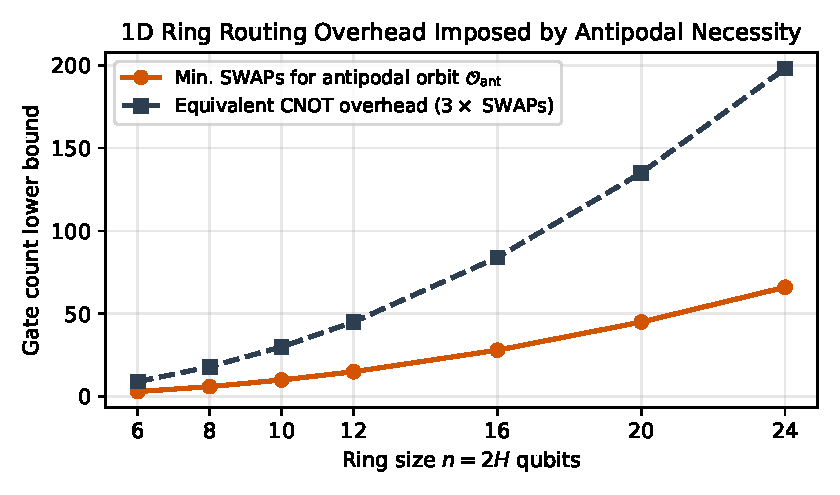
\includegraphics[width=0.72\textwidth]{figures/fig_ring_swap_overhead.pdf}
\caption{Lower bound on SWAP and equivalent CNOT routing overhead on a nearest-neighbor 1D ring ($n=2H$ qubits) imposed by Theorem~\ref{thm:antipodal} for any rotation-symmetric flat $\{Z, CZ, CCZ\}$ circuit.}
\label{fig:ring}
\end{figure}

\section{Modular Certification of Flat Degree-$\le 4$ Phase Oracles}
\label{sec:modular}

We now turn to the verification problem: given a diagonal phase circuit $U_f$ with gates in $\{Z, CZ, CCZ, CCCZ\}$ on $n = 4m$ qubits ($M = 2^m$), certify whether $\ket{\psi_f}$ is flat. Standard exact verification via the Fast Walsh--Hadamard Transform (FWHT) requires tracking integer amplitudes up to $\pm 2^n$ (at least $n/2$ bits of dynamic range around $M^2 = 2^{2m}$).

\begin{theorem}[Modular Certification of Flatness~\cite{Vono2026Rigidity}]
\label{thm:modular}
Let $n = 4m$ ($m \ge 4$), $M = 2^m$, and let $U_f$ be a diagonal phase circuit using gates in $\{Z, CZ, CCZ, CCCZ\}$ ($\deg(f) \le 4$). Let $p$ be an odd integer satisfying either
\begin{enumerate}
  \item $p \ge \frac{8}{15} M$ (valid uniformly for all $m \ge 4$), or
  \item $p \ge \frac{1}{2} M$ (valid for all $m \ge m_0$, where $m_0$ is an absolute constant).
\end{enumerate}
Then $\ket{\psi_f}$ is a flat hypergraph state if and only if
\[
  W_f(b) \equiv M^2 \quad \text{or} \quad W_f(b) \equiv -M^2 \pmod p
  \qquad \forall b \in \F_2^{4m}.
\]
\end{theorem}

\noindent\emph{Proof sketch.} Writing $X(b) = W_f(b)/M$, the congruence $W_f(b) \equiv \pm M^2 \pmod p$ forces every deviation from $|X(b)| = M$ to incur a quadratic Parseval energy penalty proportional to $pM$. Expanding the low binary digits of $X(b)$ produces low-degree Boolean discrepancy indicators whose weights are bounded below by Reed--Muller minimum-distance and Klein--Storme estimates (for $p \ge \frac{8}{15}M$) and, in the residual interval $\frac{1}{2}M \le p < \frac{8}{15}M$, by Haramaty--Shpilka structural decompositions of biased quartics for $m \ge m_0$. Whenever $f$ is non-bent, the resulting energy cost strictly exceeds the Parseval budget $\mathbb{E}_b[X(b)^2] = M^2$, yielding a contradiction~\cite{Vono2026Rigidity}.

\subsection{Overflow-Free \texttt{uint8} Modular Butterfly up to $n = 28$ Qubits}
Theorem~\ref{thm:modular} reduces the arithmetic word-width required to certify flatness from $O(n/2)$ bits to $\lceil \log_2 p \rceil \approx n/4$ bits. For $n = 16, 20, 24, 28$ qubits, the certified $8/15$ moduli are $p = 9, 19, 35, 69$, all satisfying $2p \le 255$. Representing each amplitude in $[0, p-1]$ as an unsigned 8-bit integer (\texttt{uint8}), the butterfly update
\[
  s = a + b \in [0, 2p-2], \qquad
  d = a + (p - b) \in [1, 2p-1],
\]
followed by a single conditional subtraction of $p$ whenever $s \ge p$ or $d \ge p$, is completely free of both overflow and underflow. This cuts working memory by $4\times$ relative to \texttt{int32} exact verification across all $n \le 28$ qubits (e.g., $256\,\text{MB}$ vs.\ $1024\,\text{MB}$ at $n = 28$). For $n = 32$ and $36$ qubits ($p = 137, 275$), \texttt{uint16} still provides a $2\times$ memory reduction relative to \texttt{int32} ($8\times$ relative to \texttt{complex128}), fitting $n = 36$ qubits in $128\,\text{GB}$ RAM instead of $256\,\text{GB}$ (\texttt{int32}) or $1\,\text{TB}$ (\texttt{complex128}).

\subsection{Necessity of the Threshold: Universal $p=3$ False-Positive Family}
To show that sub-threshold modular verification is fundamentally unreliable, we construct an explicit degree-$4$ circuit family that fools $p=3$ completely in every dimension $n=4m$.

\begin{proposition}[Universal $p=3$ Fooling Circuit]
\label{prop:fool}
For every $n = 4m$ ($m \ge 2$), define the degree-$4$ hypergraph circuit
\[
  f_{\mathrm{fool}}(x_0,\dots,x_{n-1})
  = \bigoplus_{i=0}^{2m-3} x_{2i} x_{2i+1}
  \;\oplus\; x_{n-4}x_{n-3}x_{n-2}x_{n-1},
\]
consisting of $2m-2$ disjoint $CZ$ gates on the first $n-4$ qubits and a single $CCCZ$ gate on the last $4$ qubits. Then:
\begin{enumerate}
  \item For every $b \in \F_2^n$, $|W_{f_{\mathrm{fool}}}(b)| \in \{\frac{7}{2}M^2, \frac{1}{2}M^2\}$, so \textbf{$0\%$ of frequencies} attain the flat magnitude $M^2$.
  \item Yet $W_{f_{\mathrm{fool}}}(b) \equiv \pm M^2 \pmod 3$ holds for \textbf{$100\%$ of all $2^n$ frequencies}.
\end{enumerate}
\end{proposition}

\begin{proof}
Since $f_{\mathrm{fool}}$ is a direct sum of a bent quadratic function on $n-4$ qubits (Walsh values $\pm 2^{2m-2} = \pm M^2/4$) and a single $4$-qubit $CCCZ$ gate (truth table of weight $1$, Walsh values $14$ at $b'=0$ and $\pm 2$ for $b'\ne 0$), the tensor-product property of $W_f$ yields $W_{f_{\mathrm{fool}}}(b) \in \{\pm \frac{7}{2}M^2, \pm \frac{1}{2}M^2\}$. Neither equals $\pm M^2$. Modulo $3$, both $14 \equiv 2 \equiv -1 \pmod 3$ and $2 \equiv -1 \pmod 3$, while $4 \equiv 1 \pmod 3$, so every coefficient satisfies $W_{f_{\mathrm{fool}}}(b) \equiv \pm 2^{2m-2} \equiv \pm 4\cdot 2^{2m-2} = \pm M^2 \pmod 3$.
\end{proof}

\section{Numerical Benchmarks}
\label{sec:benchmarks}

We implemented exact (\texttt{int32}) and overflow-free modular (\texttt{uint8}) FWHT verifiers, ring-symmetric circuit generators, and batched $2$-R\'enyi stabilizer entropy calculators in Python/NumPy, alongside a multi-threaded C/OpenMP engine for scaling to $36$ qubits.

\subsection{Modular Certification up to $n = 28$ Qubits}
Table~\ref{tab:bench} and Figure~\ref{fig:scaling} report runtime and memory scaling for degree-$4$ Maiorana--McFarland flat hypergraph circuits up to $n = 28$ qubits ($268{,}435{,}456$ amplitudes) on a standard laptop CPU ($7.7\,\text{GB}$ RAM). At $n=28$, the certified $p=69$ \texttt{uint8} verifier uses $256\,\text{MB}$ instead of $1024\,\text{MB}$ ($4\times$ reduction) and achieves a $1.35\times$ wall-clock speedup ($35.9\,\text{s}$ vs.\ $48.4\,\text{s}$) due to reduced memory bandwidth. Across $n = 16, 20, 24$, the universal fooling circuit $f_{\mathrm{fool}}$ passed $p=3$ with $0$ violations while being rejected by the certified $8/15$ modulus ($61{,}440$ violations at $n=16$; $100\%$ of frequencies at $n=20, 24$). Under random single-gate compilation fault injection ($CZ$ drops, $CZ$ misrouting, cross-register $CCZ$/$CCCZ$ insertions) at $n=16$ ($32$ faulty circuits) and $n=20$ ($13$ faulty circuits), the certified $8/15$ verifier achieved $100\%$ fault detection.

\begin{table}[h]
\centering
\footnotesize
\setlength{\tabcolsep}{4pt}
\caption{Exact (\texttt{int32}) vs.\ certified $8/15$ modular (\texttt{uint8}) flatness verification for degree-$4$ hypergraph circuits up to $n=28$ qubits.}
\label{tab:bench}
\begin{tabular}{rrrrrrr}
\toprule
$n$ & Amplitudes $2^n$ & $p_{8/15}$ ($p_{1/2}$) & Exact (ms / MB) & Mod $p_{8/15}$ (ms / MB) & Speedup & Mem. \\
\midrule
$16$ & $65{,}536$       & $9$ ($9$)   & $2.7$ / $0.25$       & $8.1$ / $0.06$      & $0.34\times$ & $4\times$ \\
$20$ & $1{,}048{,}576$  & $19$ ($17$) & $113.2$ / $4.00$     & $95.2$ / $1.00$     & $1.19\times$ & $4\times$ \\
$24$ & $16{,}777{,}216$ & $35$ ($33$) & $1564.5$ / $64.00$   & $1917.8$ / $16.00$  & $0.82\times$ & $4\times$ \\
$28$ & $268{,}435{,}456$& $69$ ($65$) & $48403.2$ / $1024.00$& $35880.3$ / $256.00$& $\mathbf{1.35\times}$ & $\mathbf{4\times}$ \\
\bottomrule
\end{tabular}
\end{table}

\begin{figure}[h]
\centering
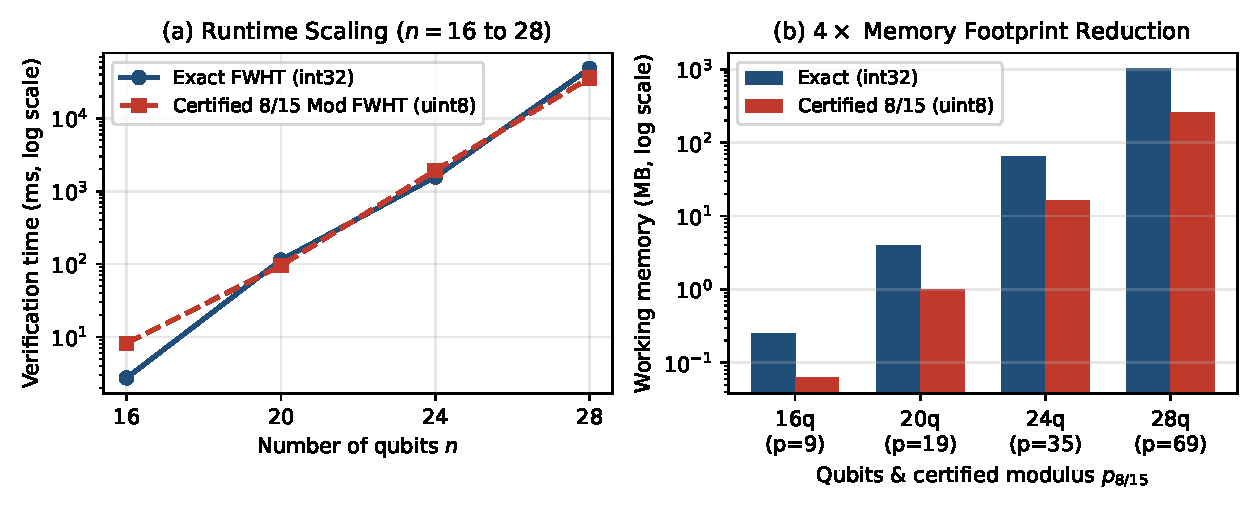
\includegraphics[width=\textwidth]{figures/fig_modular_scaling.pdf}
\caption{(a) Runtime scaling and (b) working memory footprint of exact (\texttt{int32}) vs.\ certified $8/15$ modular (\texttt{uint8}) flatness verification from $n=16$ to $n=28$ qubits.}
\label{fig:scaling}
\end{figure}

\subsection{Multi-Threaded C/OpenMP Scaling to $n = 36$ Qubits ($6.87 \times 10^{10}$ Amplitudes)}
To test memory-bandwidth-bound scaling beyond laptop RAM, we compiled our C/OpenMP engine (\texttt{gcc -O3 -march=native -fopenmp}) on cloud nodes (\texttt{n2-highmem-8} with $8$ vCPUs / $64\,\text{GB}$ RAM for $n=24,28,32$, and \texttt{n2-custom-12-163840-ext} with $12$ vCPUs / $160\,\text{GB}$ RAM and zero swap for $n=36$). Table~\ref{tab:omp32} summarizes the results. At $n = 32$ qubits ($p = 137$), certified modular verification completes in $13.67\,\text{s}$ ($1.44\times$ faster than exact \texttt{int32} at $19.74\,\text{s}$) while halving memory from $16\,\text{GB}$ to $8\,\text{GB}$. At $n = 36$ qubits ($68{,}719{,}476{,}736$ amplitudes, $p = 275$), exact \texttt{int32} verification ($256\,\text{GB}$) and standard \texttt{complex128} statevectors ($1{,}024\,\text{GB}$) exceed the $160\,\text{GB}$ node, whereas our certified \texttt{uint16} modular verifier completes in $141.57\,\text{s}$ using $128\,\text{GB}$ RAM with zero violations.

\begin{table}[h]
\centering
\footnotesize
\setlength{\tabcolsep}{3.2pt}
\caption{Multi-threaded C/OpenMP cloud benchmark up to $n = 36$ qubits ($6.87 \times 10^{10}$ amplitudes), with standard \texttt{complex128} statevector memory for reference.}
\label{tab:omp32}
\begin{tabular}{rrrrrrr}
\toprule
$n$ & $p_{8/15}$ & \texttt{complex128} & Exact \texttt{int32} (s / GB) & Mod $p_{8/15}$ (s / GB / type) & Speedup & Mem.\ vs.\ \texttt{int32} / \texttt{c128} \\
\midrule
$24$ & $35$  & $0.25\,\text{GB}$  & $0.060$ / $0.06$  & $0.042$ / $0.016$ (\texttt{uint8})  & $\mathbf{1.43\times}$ & $4\times$ / $\mathbf{16\times}$ \\
$28$ & $69$  & $4.00\,\text{GB}$  & $1.131$ / $1.00$  & $0.770$ / $0.250$ (\texttt{uint8})  & $\mathbf{1.47\times}$ & $4\times$ / $\mathbf{16\times}$ \\
$32$ & $137$ & $64.00\,\text{GB}$ & $19.739$ / $16.00$& $13.671$ / $8.000$ (\texttt{uint16})& $\mathbf{1.44\times}$ & $2\times$ / $\mathbf{8\times}$ \\
$36$ & $275$ & $1024\,\text{GB}$  & OOM / $256.00$    & $\mathbf{141.57}$ / $\mathbf{128.0}$ (\texttt{uint16}) & \textbf{feasible} & $2\times$ / $\mathbf{8\times}$ \\
\bottomrule
\end{tabular}
\end{table}

\subsection{Ring-Topology Obstruction and Quantum Magic Scaling ($n=8, 10, 12$)}
Sampling random rotation-symmetric $\{Z, CZ, CCZ\}$ circuits on $n = 6, 8, 10, 12$ qubits ($200$ samples for $n\le 10$, $60$ for $n=12$) confirmed $0\%$ flat states whenever the antipodal $CZ$ orbit $\mathcal{O}_{\mathrm{ant}}$ was omitted, in exact agreement with Theorem~\ref{thm:antipodal}. Figure~\ref{fig:magic} tracks the $2$-R\'enyi stabilizer entropy $M_2(\ket{\psi_f})$ of Maiorana--McFarland flat hypergraph states on $n=8, 10, 12$ qubits as $CCZ$ and $CCCZ$ gates are added to the $y$-register. While Clifford graph states have $M_2 = 0$, adding overlapping $CCZ$ or $CCCZ$ gates raises non-Clifford magic up to $M_2 = 2.4764$ bits while preserving exact $X$-basis flatness.

\begin{figure}[h]
\centering
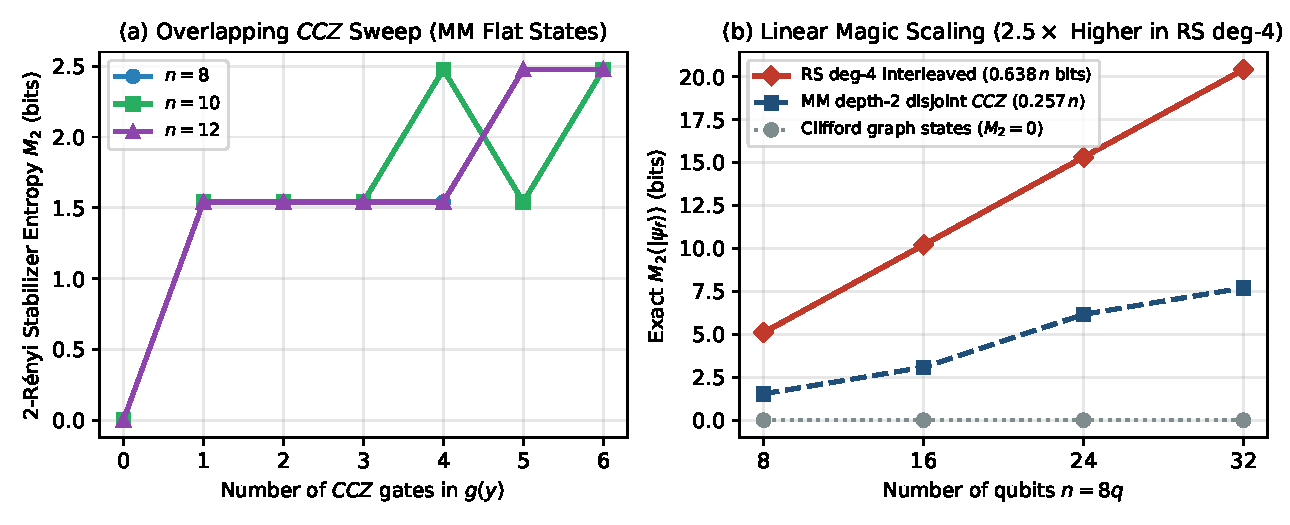
\includegraphics[width=\textwidth]{figures/fig_magic_scaling.pdf}
\caption{(a) Exact $2$-R\'enyi stabilizer entropy $M_2(\ket{\psi_f})$ under overlapping $CCZ$ gates ($n=8,10,12$), and (b) linear magic scaling across $n=8q$ qubits comparing Clifford graph states ($M_2=0$), depth-$2$ disjoint-$CCZ$ Maiorana--McFarland states ($0.257\,n$ bits), and interleaved rotation-symmetric degree-$4$ flat states ($0.638\,n$ bits, $2.5\times$ higher magic density).}
\label{fig:magic}
\end{figure}

\begin{figure}[h]
\centering
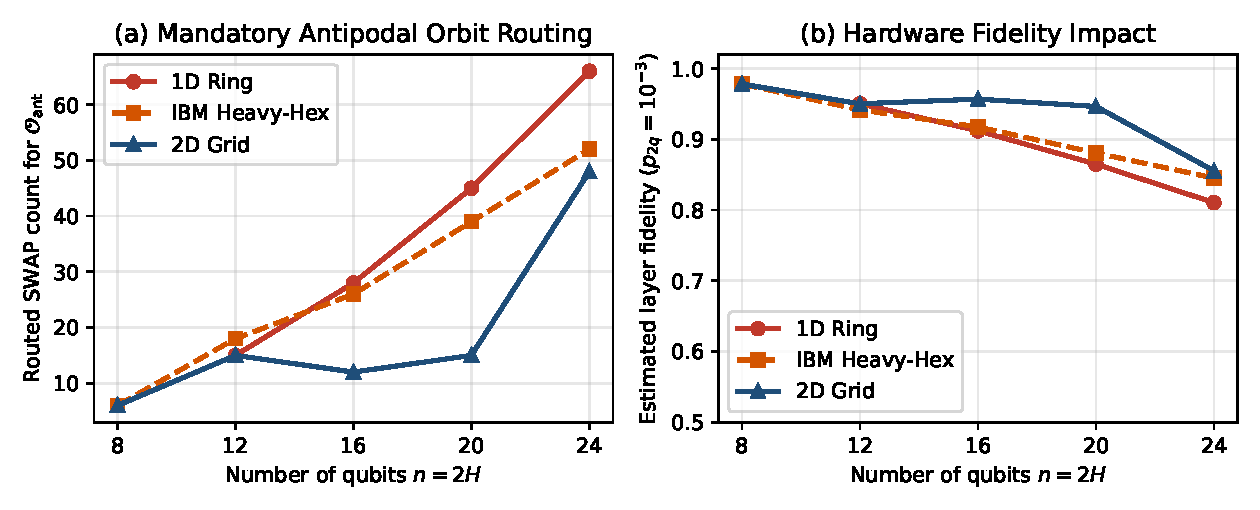
\includegraphics[width=\textwidth]{figures/fig_topology_comparison.pdf}
\caption{Greedy shortest-path SWAP routing of the mandatory antipodal orbit $\mathcal{O}_{\mathrm{ant}}$ across 1D Ring, IBM Heavy-Hex, and 2D Grid topologies ($n=8$ to $24$ qubits): (a) routed SWAP count and (b) estimated layer fidelity at $p_{2q} = 10^{-3}$.}
\label{fig:topology}
\end{figure}

\section{Exact Dimensional Reduction of Quantum Magic}
\label{sec:magic}

We now prove a self-contained quantum structural theorem showing that flat (bent) hypergraph states can achieve exact linear non-Clifford magic $M_2 = \Theta(n)$ at constant circuit depth.

\begin{theorem}[Dimensional Reduction of $M_2$ for Flat Hypergraph States]
\label{thm:magic}
Let $n = 2k$ ($k \ge 1$) and let $f(x, y) = x \cdot y \oplus g(y)$ be a Maiorana--McFarland flat hypergraph state on $n = 2k$ qubits, where $g : \F_2^k \to \F_2$ is arbitrary. Then
\[
  M_2(\ket{\psi_f}) = M_2(\ket{\psi_g}).
\]
In particular, partitioning the $k$-qubit $y$-register into $\lfloor k/3 \rfloor$ disjoint triples and applying one $CCZ$ gate per triple prepares an exact flat hypergraph state in circuit depth~$2$ with exact linear magic
\[
  M_2(\ket{\psi_f}) = \left\lfloor \frac{n}{6} \right\rfloor \log_2\!\left(\frac{32}{11}\right) \approx 0.2568\,n \text{ bits}.
\]
\end{theorem}

\begin{proof}
By construction, $\ket{\psi_f} = C\bigl(\ket{+}^{\otimes k} \otimes \ket{\psi_g}\bigr)$, where $C = \prod_{i=0}^{k-1} CZ_{i, k+i}$ is a Clifford unitary. Since the $2$-R\'enyi stabilizer entropy $M_2$ is invariant under Clifford unitaries and additive under tensor products~\cite{Leone2022}, and $M_2(\ket{+}^{\otimes k}) = 0$, we obtain $M_2(\ket{\psi_f}) = M_2(\ket{+}^{\otimes k}) + M_2(\ket{\psi_g}) = M_2(\ket{\psi_g})$. For $\lfloor k/3 \rfloor$ disjoint $CCZ$ gates on the $y$-register, $\ket{\psi_g} = \ket{\psi_{CCZ}}^{\otimes \lfloor k/3 \rfloor} \otimes \ket{+}^{\otimes (k \bmod 3)}$, and direct evaluation of the $3$-qubit $CCZ$ derivative spectrum gives $M_2(\ket{\psi_{CCZ}}) = \log_2(32/11) \approx 1.540568$ bits (and similarly $M_2(\ket{\psi_{CCCZ}}) = \log_2(512/197) \approx 1.377948$ bits for a single $CCCZ$).
\end{proof}

\subsection{NISQ Noisy $X$-Basis Flatness Testing and OpenQASM 3.0}
Combining classical modular certification (Theorem~\ref{thm:modular}, which verifies the compiler output up to $n=36$ qubits) with finite-shot $X$-basis measurements on quantum hardware yields an end-to-end verification pipeline. Figure~\ref{fig:nisq} shows a noisy simulation ($n=8$ qubits, $S=20{,}000$ shots, gate-weighted depolarizing noise $p_{2q} \in [0, 10^{-2}]$): even at $p_{2q} = 1\%$, the clean flat quartic state stays within $|Z| \le 1.22$ of uniform, whereas a single dropped $CZ$ gate ($Z = 1679$) and the universal $p=3$ fooling circuit ($Z = 5431$) are rejected at $>1600\sigma$. Ready-to-run OpenQASM~3.0 circuits are included in the repository (\texttt{qasm/}).

\begin{figure}[h]
\centering
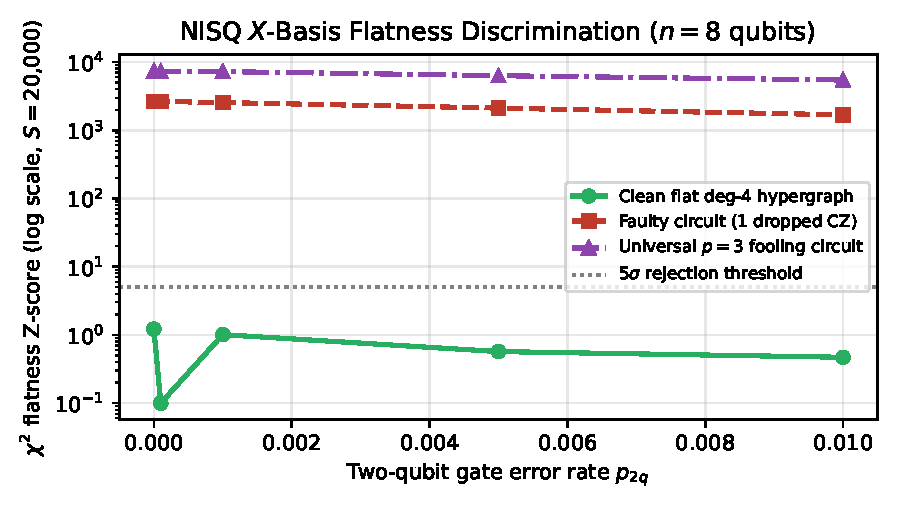
\includegraphics[width=0.76\textwidth]{figures/fig_nisq_flatness.pdf}
\caption{NISQ $X$-basis $\chi^2$ flatness Z-score ($n=8$ qubits, $S=20{,}000$ shots) across two-qubit gate error rates $p_{2q} \in [0, 0.01]$, cleanly separating flat quartic hypergraph states from single-gate compilation faults and the $p=3$ fooling circuit.}
\label{fig:nisq}
\end{figure}

\subsection{Unified Rotation-Symmetric Degree-4 Flat States ($n = 8, 16$ Qubits)}
To unite cyclic ring symmetry (Section~\ref{sec:antipodal}) and degree-4 modular certification (Section~\ref{sec:modular}) in a single circuit family, we construct an explicit rotation-symmetric degree-4 flat hypergraph state on $n=8$ qubits generated by the five cyclic orbits $\{(0,4), (0,1), (0,2), (0,1,2,4), (0,1,2,5)\}$ ($36$ gates, containing the antipodal $CZ$ orbit $(0,4)$). Direct computation yields exact $X$-basis flatness and $M_2 = 5.103668$ bits ($0.638$ bits/qubit---$2.5\times$ higher magic density than the depth-$2$ disjoint-$CCZ$ family). Interleaving $q$ disjoint copies on $n = 8q$ qubits preserves cyclic rotation symmetry, degree~$4$, and flatness; for $n=16$ ($q=2$, $72$ gates), our certified \texttt{uint8} verifier at $p = 9$ confirms exact flatness with $0$ violations and exact magic $M_2 = 10.207335$ bits. Both circuits are exported in OpenQASM~3.0 (\texttt{rs\_quartic\_flat\_n8.qasm} and \texttt{rs\_quartic\_flat\_n16.qasm}).

\section{Discussion, Reproducibility, and Disclosures}
For practical qubit counts ($n=16, 20, 24, 28$), the uniform $8/15$ bound already yields the exact same bit-width (and at $n=16$, the exact same modulus $p=9$) as the asymptotic $1/2$ bound, enabling single-byte \texttt{uint8} verification up to $28$ qubits, $13.67\,\text{s}$ verification at $32$ qubits, and $141.57\,\text{s}$ certification at $36$ qubits ($68.7$ billion amplitudes) on a single $160\,\text{GB}$ node. Natural next steps include extending modular Walsh rigidity to $\Z_4$-weighted hypergraph states ($T/S/CS$ gates) and integrating the antipodal ring obstruction as an exact pruning pass in variational compilers.

\paragraph{Scope and Limitations.}
Our modular certification theorem applies specifically to diagonal phase circuits of algebraic degree at most four ($\{Z, CZ, CCZ, CCCZ\}$, Clifford hierarchy levels $\mathcal{C}_1$--$\mathcal{C}_4$) rather than arbitrary universal circuits with interleaved non-diagonal gates. Moreover, exhaustive classical verification remains $O(n 2^n)$ in frequency count: the modular engine provides a constant-factor reduction in word-width ($4\times$ vs.\ \texttt{int32} and $16\times$ vs.\ \texttt{complex128} up to $28$ qubits; $2\times$ / $8\times$ at $32$--$36$ qubits) that extends the practical classical verification frontier by $1$--$3$ qubits (and accelerates block-wise compiler verification), whereas the antipodal ring obstruction (Theorem~\ref{thm:antipodal}) and linear magic constructions (Theorem~\ref{thm:magic}) scale analytically to arbitrary qubit counts.

\paragraph{Code and Data Availability.}
All Python/NumPy simulation scripts, the multi-threaded C/OpenMP $36$-qubit engine (\texttt{src/fwht\_omp.c}), OpenQASM~3.0 circuits (\texttt{qasm/}), and JSON benchmark logs (\texttt{results/}) are packaged for full reproducibility.

\paragraph{AI-Assistance Disclosure.}
AI coding and analytical assistants were used to help draft code, execute numerical benchmarks, and format the manuscript; all mathematical statements, theorem citations, and numerical outputs were independently verified against exact computations and the cited formal/analytical preprints.

\begin{thebibliography}{10}
\bibitem{Vono2026Antipodal}
F.~M.~Vono,
\emph{Antipodal Necessity and the Cubic Case of the Homogeneous Rotation-Symmetric Bent Function Conjecture},
Figshare preprint (Version~2), 2026.
\url{https://doi.org/10.6084/m9.figshare.34165260.v2}

\bibitem{Vono2026Rigidity}
F.~M.~Vono, A.~O.~N.~de Toledo, and V.~G.~Santos,
\emph{Modular Walsh rigidity for Boolean functions of degree at most four: the $1/2$ bound in large dimensions},
Figshare preprint (Version~4), 2026.
\url{https://doi.org/10.6084/m9.figshare.34963642.v4}

\bibitem{Gottesman1999}
D.~Gottesman and I.~L.~Chuang,
\emph{Demonstrating the viability of universal quantum computation using teleportation and single-qubit operations},
Nature \textbf{402}, 390--393 (1999).

\bibitem{Cui2017}
S.~X.~Cui, D.~Gottesman, and A.~Krishna,
\emph{Diagonal gates in the Clifford hierarchy},
Physical Review A \textbf{95}, 012329 (2017).

\bibitem{Rossi2013}
M.~Rossi, M.~Huber, D.~Bru\ss, and C.~Macchiavello,
\emph{Quantum hypergraph states},
New Journal of Physics \textbf{15}, 113022 (2013).

\bibitem{Qu2013}
R.~Qu, J.~Wang, Z.-s.~Li, and Y.-r.~Bao,
\emph{Encoding hypergraphs into quantum states},
Physical Review A \textbf{87}, 022311 (2013).

\bibitem{Gachechiladze2019}
M.~Gachechiladze, O.~G\"uhne, and A.~Miyake,
\emph{Changing the facet of multipartite entanglement with hypergraph states},
Physical Review A \textbf{99}, 052304 (2019).

\bibitem{Rotteler2010}
M.~R\"otteler,
\emph{Quantum algorithms for highly non-linear Boolean functions},
Proc.\ 21st Annual ACM--SIAM Symposium on Discrete Algorithms (SODA), 448--457 (2010).

\bibitem{Leone2022}
L.~Leone, S.~F.~E.~Oliviero, and A.~Hamma,
\emph{Stabilizer R\'enyi Entropy},
Physical Review Letters \textbf{128}, 050402 (2022).

\bibitem{Carlet2021}
C.~Carlet,
\emph{Boolean Functions for Cryptography and Coding Theory},
Cambridge University Press, 2021.
\end{thebibliography}

\end{document}
